\section{Part II: The Evolution of Tool-Augmented Task Execution}
\headingnote{From ``Experimental Tool User'' to ``Workstation Expert''}

This part shifts the focus from the model's internal cognition to its external ability to act.
Once LLMs acquire stronger reasoning capabilities, the next question is whether they can use that cognition to operate tools, interact with environments, and complete external tasks~\citep{autogpt2023,babyagi2023,anthropic2024claude35haiku,mialon2023gaia,mcp2026servers}.
We first revisit the Agent era, where perception, planning, memory, and tool invocation are organized into an environment--action--feedback loop.
We then examine the OpenClaw era, where this loop is embedded into persistent workspaces with reusable skills, stateful execution, and stronger requirements for task closure, reliability, and governance~\citep{singh2025agentic,huang2024understanding,dong2024survey,yehudai2025survey,mamun2026anatomical,liu2026knowledge,dong2025youtu}.


\subsection{The Agent Era: Environment--Action--Feedback Loops}
\headingnote{General Intelligent Body: tool invocation and initial autonomy}

As shown in Figure~\ref{fig:agent}, the Agent era marks the first major attempt to turn LLMs from passive conversational systems into active problem solvers.
Instead of producing a single answer and stopping, an agent observes an environment, reasons about the next step, invokes a tool or action, receives feedback, and iterates.
This loop gives LLMs an initial form of autonomy: they can search, call APIs, write code, browse pages, remember intermediate information, and adjust plans from external results~\citep{zhao2023depth,xu2025llm,yang2026toward,xie2024large,cao2025large}.
However, this autonomy remains fragile because the environment is still treated as a sequence of disconnected tool responses rather than as a persistent workspace.
We therefore review the core capabilities that define this era, followed by the evaluation evidence and structural bottlenecks that motivate the transition to OpenClaw-style workstation agents.

\begin{figure}[t]
    \centering
    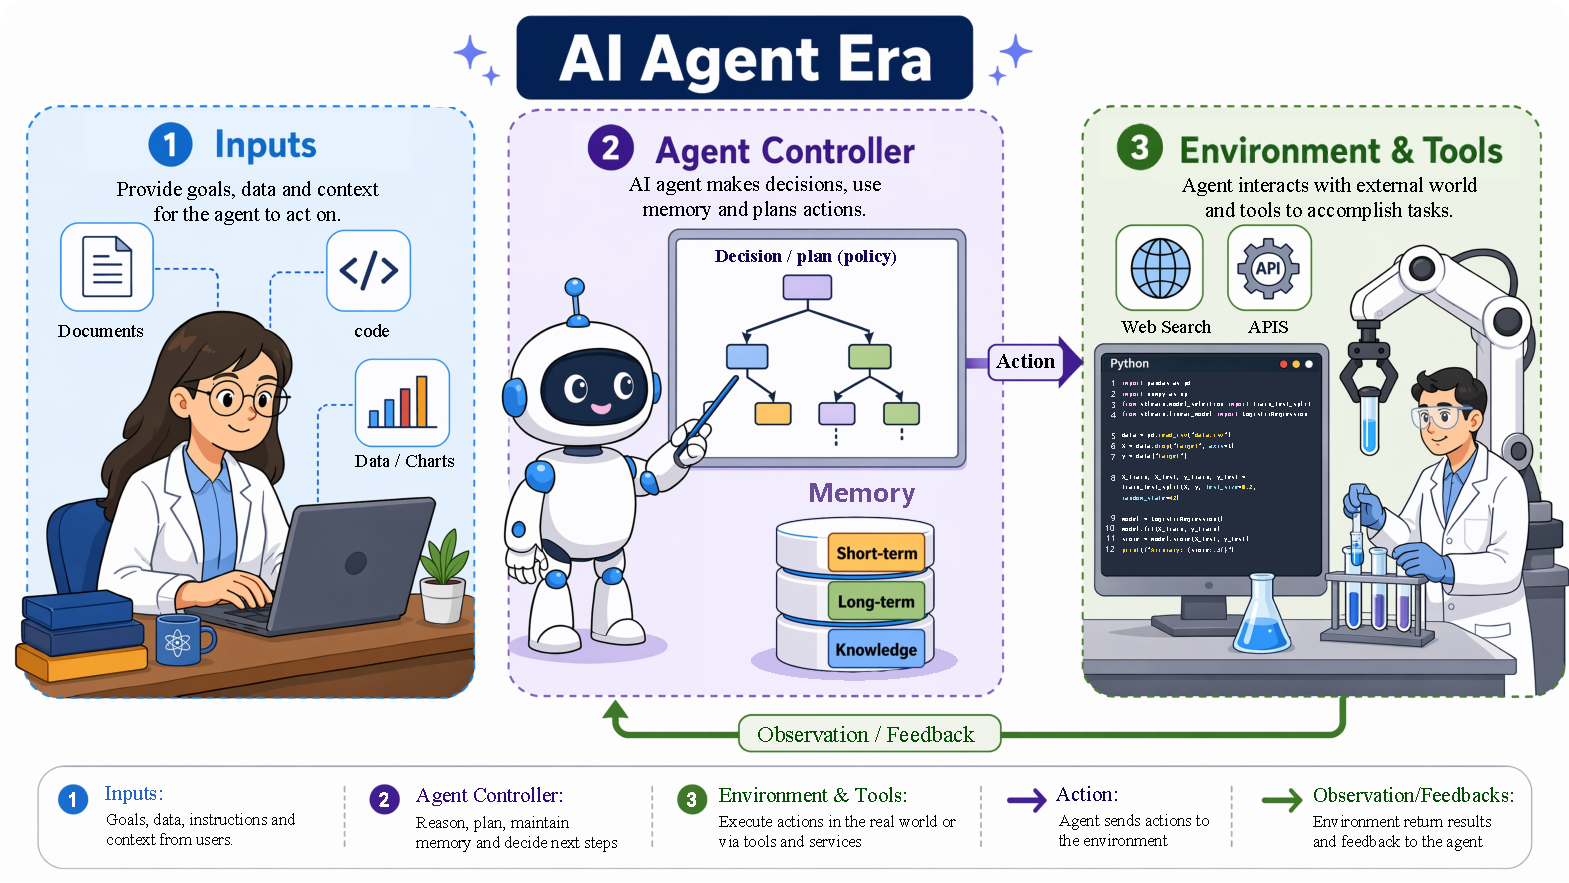
\includegraphics[width=\textwidth]{figure/agent.pdf}
    \caption{The Agent Era: the model observes an external environment, plans the next step, invokes tools or actions, receives feedback, and iterates toward the task goal. The figure illustrates the observe--think--act--observe loop that gives LLMs an initial form of autonomy beyond single-turn answering.}
    \label{fig:agent}
\end{figure}


\subsubsection{Tool Invocation and Core Agent Capabilities}

\textbf{Agentic Interaction Loop.} The Agent era marks the first organized and systematic effort to extend pretrained LLMs from single-turn question answering into sustained, multi-step interaction with complex external environments. Different from traditional LLMs, the agent operates within an environment loop, observing the world, selecting actions that may invoke external tools, receiving feedback, and iterating. This closed loop of observing, thinking, acting, and observing again is what fundamentally distinguishes an agent from a chatbot. ReAct \cite{yao2022react} established the canonical form of this loop by interleaving \emph{Thought}, \emph{Action}, and \emph{Observation} in an alternating chain, demonstrating that synergizing reasoning and acting outperforms either in isolation on knowledge-intensive and decision-making tasks. The pattern became so influential that nearly every later agent system can be read as an extension, refinement, or specialization of the ReAct loop~\citep{ruan2023tptu,lee2026survey,shen2024llm,li2024survey,NEURIPS2025_48dcc43a}.

\textbf{Agent Architecture.} Several influential frameworks have sought to formalize what makes a system an agent rather than merely an LLM with tools. Wang et al. \cite{wang2024survey} proposed a four-module architecture consisting of \emph{Profile}, \emph{Memory}, \emph{Planning}, and \emph{Action}, establishing the vocabulary that subsequent work has largely adopted. Xi et al. \cite{xi2023rise} approached the same question from cognitive science, drawing parallels between LLM agents and theories of human cognition. The CoALA framework \cite{sumers2023cognitive} further refined this direction by mapping agent capabilities onto constructs from cognitive psychology, including working memory and long-term memory such as episodic, semantic, and procedural memory, as well as a decision-making cycle. More recently, Buyya et al. \cite{buyya2026agentic} identified six modular dimensions of LLM agents, including \emph{Perception}, \emph{Memory}, \emph{Action}, \emph{Planning}, \emph{Reflection}, and \emph{Learning}, offering a control-theoretic lens through a POMDP formulation that complements the cognitive perspective. Despite terminological differences, these frameworks converge on four essential capabilities. \emph{Perception} refers to observing and interpreting the environment. \emph{Planning} involves decomposing goals and reasoning about action sequences. \emph{Memory} concerns maintaining context and accumulating experience. \emph{Tool use} means invoking external APIs to effect change. We trace these developments below~\citep{li2025review,xu2026evolution,xi2026toolgym,chezelles2024browsergym,kruppweb,wu2026omniflowphysicsgroundedmultimodalagent,11356944,ICLR2024_d53538ba,dong2026deep}.

\textbf{Perception.} An agent's effectiveness is fundamentally bounded by what it can observe. Early agents operated in purely textual environments, parsing structured outputs from APIs or web scrapers. A first generation of multi-modal perception delegated sensory processing to external specialist models orchestrated by the LLM. For example, HuggingGPT \cite{shen2023hugginggpt} treats the LLM as a controller that selects models from the Hugging Face ecosystem for sub-tasks such as image captioning and object detection. Along similar lines, Visual ChatGPT \cite{wu2023visual} chains visual foundation models via a prompt manager to handle diverse visual interactions. Taking a program-synthesis approach, ViperGPT \cite{suris2023vipergpt} generates Python programs that compose vision-API calls for compositional visual reasoning. While effective as proof-of-concept demonstrations, these indirect pipelines suffer from error compounding, since each specialist model introduces its own failure modes and the LLM has no direct access to raw sensory signals. The emergence of powerful vision language models has since enabled agents to perceive environments directly through screenshots. Set-of-Mark (SoM) prompting \cite{yang2023set} overlays numbered markers onto UI elements, enabling GPT-4V to refer to specific interface components by index. A dedicated line of GUI agents has pushed this further: CogAgent \cite{hong2024cogagent} employs a dual-resolution visual encoder for fine-grained UI recognition, ShowUI \cite{lin2025showui} unifies vision, language, and action in a single model that directly outputs UI operations from screenshots, and UI-TARS \cite{qin2025ui} achieves context-aware understanding of both desktop and mobile interfaces through large-scale GUI training. Despite these advances, agent perception remains fragmented: most agents observe one snapshot at a time, without persistent visual working memory across steps and tasks~\citep{guo2026mcp,ahn2026orchestrationbench,ding2026wildclawbench,hu2026agentic,li2026benchmark,koh2024visualwebarena,rawles2025androidworld,wang2024mobile,zhang2025appagent,cheng2024seeclick,10.1145/3690642,dong2026deep, zhang2026ssrb, huang2025deepresearchguard}.

\textbf{Planning.} Planning, broadly defined as the ability to break a complex goal into achievable sub-steps and recover when things go wrong, has progressed through several generations \cite{li2025towards,li2025benchmarking, kuang2026atomic, guo2026evoconfig}. The foundational insight came from Chain-of-Thought (CoT) prompting \cite{wei2022chain}, which demonstrated that generating intermediate reasoning steps dramatically improves multi-step performance and now forms the backbone of most agent planning systems. Building on this foundation, Tree of Thoughts (ToT) \cite{yao2023tree} extended the paradigm by allowing multiple reasoning branches and backtracking, effectively casting planning as a search problem. Graph of Thoughts (GoT) \cite{besta2024graph} generalized this idea further by supporting arbitrary graph topologies over reasoning steps. Complementary to search-based methods is the strategy of task decomposition. Decomposed Prompting \cite{khot2022decomposed} breaks problems into modular sub-problems handled by specialized prompts, while Least-to-Most Prompting \cite{zhou2022least} takes an incremental approach by solving progressively harder sub-problems, using earlier solutions as building blocks. Beyond forward planning, a distinguishing feature of effective agents is their capacity for in-episode learning from failure. Reflexion \cite{shinn2023reflexion} addresses this by generating natural-language reflections on failed attempts and incorporating them into subsequent tries. Similarly, Self-Refine \cite{madaan2023selfrefine} uses iterative self-feedback to improve outputs without external supervision. Taking a more formal approach, Reasoning via Planning (RAP) \cite{hao2023reasoning} brings classical search into the picture by combining Monte Carlo Tree Search with the LLM serving as both world model and value function. More recently, a paradigm shift has emerged through the use of reinforcement learning to train models that autonomously interleave reasoning with tool use at inference time.

\textbf{Memory.} LLMs are fundamentally stateless, as each inference call starts with a blank slate and the only memory available is whatever fits within the context window~\cite{packer2023memgpt,wang2023augmenting,shan2025cognitive,fang2025lightmem,du2026memory}. For agents operating over extended horizons, this poses a severe limitation. A useful cognitive framing distinguishes semantic, episodic, and procedural memory: agents must access external knowledge, preserve task experiences, and reuse learned procedures over time \cite{zhang2025survey,pink2025position}. In practice, agent memory has moved from retrieval-based knowledge access to persistent experience accumulation, multimodal environmental memory, and scalable learned management~\citep{li2026world,zhu2025evolutionary,qin2025aptbench,jiang2026sok,adamenko2025swe}.

Moving beyond retrieval, Generative Agents \cite{park2023generative} introduced the influential memory stream architecture, where agents record observations as timestamped entries and periodically synthesize high-level reflections from low-level experiences. Subsequent work explored more structured forms of long-term memory: MemoryBank \cite{zhong2024memorybank} proposed persistent memory with forgetting mechanisms, while ChatDB \cite{hu2023chatdb} used databases as symbolic external memory accessible via SQL. These systems shift memory from external knowledge access to persistent experience accumulation~\citep{deng2025swe,zhang2026swe,tian2026swe,rashid2025swe,badertdinov2026swe}.

Drawing on cognitive science, the Memory Mechanism Survey \cite{zhang2025survey} provides a systematic taxonomy distinguishing between semantic, episodic, and procedural memory for agents, and the Episodic Memory position paper \cite{pink2025position} further argues that episodic memory is the missing piece for maintaining logical consistency across extended interactions. This framing clarifies that agent memory is not a monolithic storage buffer, but a set of distinct mechanisms for preserving facts, experiences, procedures, and self-consistency~\citep{aleithan2024swe,yang2026swe,wang2025swe,sonwane2026omnicode,garg2025saving}.

As autonomous agents become increasingly multimodal, their memory must also preserve perceptual experience rather than only textual interaction histories. MEIA \cite{liu2024meia} introduces a multimodal environmental memory that stores object-level, spatial, and temporal information for embodied agents. MIRIX \cite{wang2025mirix} proposes a modular multi-agent memory system covering semantic, episodic, procedural, and resource memories across heterogeneous text and visual inputs. M3-Agent \cite{long2025seeing} further studies long-term multimodal memory for agents that perceive visual and auditory streams, showing how such memories can support future reasoning and downstream interaction~\citep{ma2025swe,he2025swe,peng2025swe,han2026swe,prathifkumar2025does}.

More recently, a new generation of production-scale systems has advanced agent memory toward practical deployment. Mem0 \cite{chhikara2025mem0} implements a scalable memory-centric architecture achieving 91\% lower p95 latency and over 90\% token cost savings compared to full-context baselines, and its enhanced variant Mem0g introduces graph-based representations to capture relational structure. Taking a different perspective, A-MEM \cite{xu2026mem} draws inspiration from the Zettelkasten method, enabling agents to build interconnected knowledge networks through dynamic indexing and linking. Perhaps most significantly, reinforcement learning is now being applied to teach agents how to manage their own memory autonomously. MEM1 \cite{zhou2025mem1} enables agents to operate with constant memory across long multi-turn tasks through end-to-end RL, achieving 3.5$\times$ performance improvement while reducing memory usage by 3.7$\times$. Along a complementary line, Memory-R1 \cite{yan2025memory} trains a Memory Manager with structured operations (ADD, UPDATE, DELETE, NOOP) using only 152 training pairs, yet outperforms strong baselines across three benchmarks. Mem-$\alpha$ \cite{wang2025mem} and MemMachine \cite{wang2026memmachine} represent further points in this design space, with the former learning memory construction via RL and the latter preserving factual integrity through sentence-level episode storage. The trend is clear: memory is evolving from static retrieval and heuristic storage into an adaptive capability for knowledge access, multimodal experience, and long-horizon context management~\citep{applis2025unified,lai2024autowebglm,patel2024large,thil2024navigating,anupam2025browserarena}.

\textbf{Tool Use.} If perception is the agent's eyes and systematic planning its brain, then tool use is its hands: it is the mechanism through which large language models (LLMs) translate internal reasoning into tangible external operations. The paradigm shift of tool use in LLM agents is understood as a progression from executable calls to large-scale API grounding, long-horizon trajectory-level control, and standardized tool infrastructures~\citep{chae2025web,krupp2025quantifying,xu2025turkingbench,murty2024nnetnav,lu2024weblinx,wang2024executable,chen2023fireact}.

The first problem is \emph{executable tool use}: how can a large language model move beyond textual answers and produce operations that can be successfully executed by an external system? Early tool-integrated reasoning methods established this crucial bridge between language generation and execution. Toolformer~\cite{schick2023toolformer} proposed a self-supervised approach that augments text with tool calls at positions where external tools improve prediction, enabling the model to learn when and how to invoke tools. PAL~\cite{gao2023pal} and Program of Thoughts (PoT)\cite{chen2022program} take code execution as a meta-tool: the model generates executable programs while exact computation is delegated to an interpreter. These works mark the first step beyond pure text generation: the model can effectively externalize its reasoning into an executable substrate\citep{cai2025large,song2025bearcubs,zhang2024large,caples2026real,bhathal2025websight}.

Once successful tool invocation becomes possible, the primary bottleneck shifts from \emph{whether} a model can call a tool to \emph{which} tool it should call and \emph{how} the call should be constructed. This gives rise to the problem of \emph{API grounding at scale}. In complex realistic environments, tools are not a small hand-written set of functions but large API ecosystems with complex documentation, argument schemas, and usage constraints. Gorilla~\cite{patil2023gorilla} addresses this problem by fine-tuning LLMs on API documentation, enabling them to generate accurate calls for both familiar and unseen endpoints. ToolLLM~\cite{qin2023toolllm} scales this direction with ToolBench, a benchmark containing over 16,000 real-world RESTful APIs across 49 categories, and introduces search-based decision procedures for selecting and chaining tools. ToolACE~\cite{liu2025toolace} further shows that high-quality synthetic tool-calling data can produce compact language models with strong zero-shot function-calling ability. This work reframes tool use as interface grounding: the model must map intent to the right API, respect schemas, and produce valid arguments~\citep{pan2024webcanvas,trabucco2025towards,hu2025agentgen,wang2023describe,cheng2024exploring,zhuang2023toolqa,huang2024metatool,guo2024stabletoolbench,du2024anytool,song2023restgpt,miao2025recode}.

However, correct local calls do not by themselves produce reliable agents. In multi-step tasks, tool use becomes a \emph{trajectory-level control} problem. The agent must decide when external execution is necessary, avoid unnecessary calls, incorporate tool feedback, recover from failed executions, and stop when the task is complete. SMART~\cite{qian2025smart} studies this issue from the perspective of tool overuse, training agents to balance parametric reasoning with external tool dependence. START~\cite{li2025start} shows that tool-integrated reasoning traces can be bootstrapped through hint-based self-learning rather than relying only on manually written demonstrations. Reinforcement-learning-based methods push this direction further by treating tool invocation as part of the rollout environment. ReTool~\cite{feng2025retool} trains models to interleave natural-language reasoning with real-time code execution, while ToRL~\cite{li2025torl} scales tool-integrated reinforcement learning with code interpreters inside the rollout process. ToolRL~\cite{qian2026toolrl} highlights the importance of reward design, especially the granularity and temporal structure of rewards for tool selection and application. ARTIST~\cite{singh2505agentic}, Tool-Star~\cite{dong2505tool}, and AutoTIR~\cite{wei2025autotir} extend this line toward multi-turn or multi-tool settings, where models coordinate reasoning, invocation, and execution feedback within one trajectory. The central shift is from isolated tool calls to policies that control tool use over time~\citep{xi2025agentgym,mahdavi2024leveraging,li2025exploring,gao2024large,birr2024autogpt+,basu2024api,ye2025tooleyes,gao2024confucius,wang2024gta}.

As tool-augmented agents move toward commercial deployment, the primary bottleneck shifts again from model-side tool use to infrastructure-level standardization. Fragmented tool interfaces make agents difficult to scale, secure, and govern, because each tool may expose different schemas, authentication mechanisms, context formats, and execution constraints. The Model Context Protocol (MCP)\cite{mcp2026tools}, introduced by Anthropic in November 2024, represents a coordinated effort to standardize how LLMs connect to external tools and data sources, analogous to how common peripheral protocols standardize hardware connectivity. Since its release, both OpenAI and Google have announced MCP support, signaling a trend toward industry-wide convergence. In parallel, major commercial LLM APIs now widely support native function calling as a first-class interface, moving tool invocation from ad-hoc prompting toward structured execution\citep{hu2023language,babu2025adaptive,li2025task,wang2023describe,huang2025recommender}.

The overall trajectory is therefore not simply from fewer tools to more tools. Rather, tool use evolves from executable calls to grounded API use, from locally valid calls to trajectory-level tool-use policies, and from fragmented interfaces to standardized tool infrastructures. This progression also exposes the boundary of the Agent era. Tool use gives agents the ability to act, but the effects of these actions often remain fragmented across isolated calls and transient tool responses. The next step, developed in the OpenClaw era, is to embed tool use inside persistent workspaces where files, sessions, skills, logs, permissions, and verification procedures can support durable task closure in real deployments.





\subsubsection{Initial Autonomy: Evaluation and Structural Bottlenecks}

To assess the practical reliability of LLM-based agents, several benchmarks have been developed. AgentBench \cite{liu2023agentbench} evaluates agents across eight environments, revealing a performance gap between commercial and open-source models in multi-step settings. WebArena \cite{zhou2023webarena} uses realistic web environments where GPT-4 achieved only ~14\% success. SWE-bench \cite{jimenez2023swebench} focuses on GitHub issue resolution for coding, while GAIA \cite{mialon2023gaia} tests general assistants on multi-step reasoning and tool use. Across these benchmarks, success rates decay super-linearly with complexity and horizon length, prompting systematic failure analysis. The LLM Agent Failure study \cite{roig2025llms} identifies four archetypes: premature ungrounded action, over-helpfulness with plausible but incorrect details, distractor-induced context pollution, and fragile execution under load. Similarly, the Agent Hallucination survey \cite{lin2025llm} notes that "hallucinated actions"—such as calling incorrect APIs or operating wrong files—cause irreversible failures, unlike text-level hallucinations~\citep{he2024webvoyager,yoran2024assistantbench,wu2024copilot,zhang2025ufo,huang2023mlagentbench, kuang2025process, ye2025productagent}.

Synthesizing the empirical evidence from existing benchmarks and failure analyses, we identify four critical structural bottlenecks of the Agent era:
\begin{itemize}
    \item \textbf{Fragmented perception.} Agents observe the environment through narrow, episodic windows---a single API response, a single screenshot, a single tool output. They lack a persistent, holistic model of the environment's state and how it evolves over time.
    \item \textbf{Ephemeral tool invocation.} Each tool call is an isolated transaction. No stable workspace exists where intermediate artifacts persist: files created in one step may be inaccessible in the next; terminal sessions are not preserved; browser state is lost between actions.
    \item \textbf{Brittleness under environmental uncertainty.} Real-world environments are noisy, asynchronous, and adversarial. Network timeouts, UI changes, API responses, and permission errors compound across long sequences, sharply lowering success rates.
    \item \textbf{Absence of long-term task closure.} Agents can attempt tasks but rarely complete them reliably end-to-end. They lack the persistent state, error recovery mechanisms, and verification loops needed to deliver finished work products rather than best-effort attempts.
\end{itemize}

These bottlenecks are not mere engineering issues solved by prompting or scaling, but a fundamental architectural limitation: current agents treat environments as external oracles to query, rather than persistent workspaces to inhabit. Overcoming this requires shifting from tool-calling agents to agents working inside workstations. Here, we strictly define LLM-based agents as systems operating through an environment-action-feedback loop with external tools. Earlier techniques—like chain-of-thought, retrieval-augmented generation, and memory—are not agents themselves, but foundational capabilities. Table~\ref{tab:agent_era} summarizes both agent systems and these enabling capabilities.

\begin{table}[htbp]
\centering
\scriptsize
\setlength{\tabcolsep}{8pt}
\renewcommand{\arraystretch}{1.1}
\caption{Representative works related to LLM-based agents and their enabling capabilities.}
\label{tab:agent_era}
\resizebox{\columnwidth}{!}{
\begin{tabular}{@{} l l l l l @{}}
\toprule
\textbf{Work} & \textbf{Year} & \textbf{Category} & \textbf{Role} & \textbf{Key Contribution} \\
\midrule

ReAct~\cite{yao2022react} & 2022 & Agent Architecture & Agent Framework & Thought--Action--Observation loop \\
Wang et al.~\cite{wang2024survey} & 2024 & Agent Architecture & Conceptual Framework & Profile/Memory/Planning/Action architecture \\
Xi et al.~\cite{xi2023rise} & 2023 & Agent Architecture & Conceptual Framework & Cognitive-science perspective on agents \\
CoALA~\cite{sumers2023cognitive} & 2023 & Agent Architecture & Conceptual Framework & Cognitive psychology mapping for agents \\
Buyya et al.~\cite{buyya2026agentic} & 2026 & Agent Architecture & Conceptual Framework & Six dimensions with POMDP formulation \\
HuggingGPT~\cite{shen2023hugginggpt} & 2023 & Perception & Agent System & LLM orchestrating Hugging Face models \\
Visual ChatGPT~\cite{wu2023visual} & 2023 & Perception & Agent System & Chaining visual models via prompt manager \\
ViperGPT~\cite{suris2023vipergpt} & 2023 & Perception & Agent System & Program synthesis for visual reasoning \\
Set-of-Mark~\cite{yang2023set} & 2023 & Perception & Enabling Capability & Numbered markers for UI grounding \\
CogAgent~\cite{hong2024cogagent} & 2024 & Perception & Agent Model & Dual-resolution encoder for UI recognition \\
ShowUI~\cite{lin2025showui} & 2025 & Perception & Agent Model & Unified vision--language--action for UI ops \\
UI-TARS~\cite{qin2025ui} & 2025 & Perception & Agent Model & Context-aware desktop/mobile GUI understanding \\
CoT~\cite{wei2022chain} & 2022 & Planning & Enabling Capability & Intermediate reasoning steps \\
ToT~\cite{yao2023tree} & 2023 & Planning & Enabling Capability & Multi-branch reasoning with backtracking \\
GoT~\cite{besta2024graph} & 2024 & Planning & Enabling Capability & Graph topologies over reasoning steps \\
Decomposed Prompting~\cite{khot2022decomposed} & 2022 & Planning & Enabling Capability & Modular sub-problem decomposition \\
Least-to-Most~\cite{zhou2022least} & 2022 & Planning & Enabling Capability & Incremental sub-problem solving \\
Reflexion~\cite{shinn2023reflexion} & 2023 & Planning & Agent Framework & Language reflections on failed attempts \\
Self-Refine~\cite{madaan2023selfrefine} & 2023 & Planning & Enabling Capability & Iterative self-feedback improvement \\
RAP~\cite{hao2023reasoning} & 2023 & Planning & Enabling Capability & MCTS with LLM as world model \\
Search-R1~\cite{jin2025search} & 2025 & Planning & Agent Model & RL-trained search in reasoning chains \\
R1-Searcher~\cite{song2025r1} & 2025 & Planning & Agent Model & Two-stage RL for search--reasoning \\
ReSearch~\cite{chen2503research} & 2025 & Planning & Agent Model & Supervision-free RL with search ops \\
RAG~\cite{lewis2020retrieval} & 2020 & Memory & Enabling Capability & Retrieval-augmented generation \\
Self-RAG~\cite{asai2024self} & 2024 & Memory & Enabling Capability & Adaptive retrieval with self-reflection \\
CRAG~\cite{yan2024corrective} & 2024 & Memory & Enabling Capability & Retrieval evaluation and correction \\
Adaptive-RAG~\cite{jeong2024adaptive} & 2024 & Memory & Enabling Capability & Strategy routing by query complexity \\
Generative Agents~\cite{park2023generative} & 2023 & Memory & Agent System & Memory stream with reflections \\
MemoryBank~\cite{zhong2024memorybank} & 2024 & Memory & Enabling Capability & Persistent memory with forgetting \\
ChatDB~\cite{hu2023chatdb} & 2023 & Memory & Enabling Capability & Database as external memory via SQL \\
MEIA~\cite{liu2024meia} & 2024 & Memory & Agent System & Multimodal environmental memory \\
MIRIX~\cite{wang2025mirix} & 2025 & Memory & Memory Infrastructure & Multi-agent multimodal memory system \\
M3-Agent~\cite{long2025seeing} & 2025 & Memory & Agent System & Long-term visual-auditory memory \\
Memory Survey~\cite{zhang2025survey} & 2025 & Memory & Conceptual Framework & Semantic/episodic/procedural taxonomy \\
Episodic Memory~\cite{pink2025position} & 2025 & Memory & Conceptual Framework & Position paper on episodic consistency \\
Mem0~\cite{chhikara2025mem0} & 2025 & Memory & Memory Infrastructure & Scalable memory; graph-based Mem0g \\
A-MEM~\cite{xu2026mem} & 2026 & Memory & Memory Infrastructure & Zettelkasten-inspired knowledge networks \\
MEM1~\cite{zhou2025mem1} & 2025 & Memory & Agent Model & End-to-end RL for constant memory \\
Memory-R1~\cite{yan2025memory} & 2025 & Memory & Agent Model & RL-trained structured memory manager \\
Mem-$\alpha$~\cite{wang2025mem} & 2025 & Memory & Agent Model & Memory construction via RL \\
MemMachine~\cite{wang2026memmachine} & 2026 & Memory & Memory Infrastructure & Sentence-level episode storage \\
Toolformer~\cite{schick2023toolformer} & 2023 & Tool Use & Agent Model & Self-supervised tool-call learning \\
PAL~\cite{gao2023pal} & 2023 & Tool Use & Enabling Capability & Code execution as meta-tool \\
PoT~\cite{chen2022program} & 2022 & Tool Use & Enabling Capability & Multi-step reasoning via programming \\
Gorilla~\cite{patil2023gorilla} & 2024 & Tool Use & Agent Model & Fine-tuning on API documentation \\
ToolLLM~\cite{qin2023toolllm} & 2023 & Tool Use & Agent Framework & 16K+ APIs; DFS-based decision trees \\
SMART~\cite{qian2025smart} & 2025 & Tool Use & Agent Model & Tool overuse mitigation \\
START~\cite{li2025start} & 2025 & Tool Use & Agent Model & Self-taught tool-integrated reasoning \\
ReTool~\cite{feng2025retool} & 2025 & Tool Use & Agent Model & RL for strategic tool invocation \\
ToRL~\cite{li2025torl} & 2025 & Tool Use & Agent Model & Tool-integrated RL with code execution \\
ToolRL~\cite{qian2026toolrl} & 2026 & Tool Use & Agent Model & Reward design for tool learning \\
ARTIST~\cite{singh2505agentic} & 2025 & Tool Use & Agent Model & Agentic reasoning with tool integration \\
Tool-Star~\cite{dong2505tool} & 2025 & Tool Use & Agent Model & Multi-tool reasoning via RL \\
AutoTIR~\cite{wei2025autotir} & 2025 & Tool Use & Agent Model & Autonomous tool-integrated reasoning \\
MCP~\cite{mcp2026tools} & 2024 & Tool Use & Infrastructure & Universal LLM--tool connectivity protocol \\
ToolACE~\cite{liu2025toolace} & 2025 & Tool Use & Agent Model & Synthesized data for compact tool callers \\
AgentBench~\cite{liu2023agentbench} & 2023 & Benchmark & Evaluation & 8-environment agent evaluation \\
WebArena~\cite{zhou2023webarena} & 2023 & Benchmark & Evaluation & Realistic web task environments \\
SWE-bench~\cite{jimenez2023swebench} & 2024 & Benchmark & Evaluation & GitHub issue resolution benchmark \\
GAIA~\cite{mialon2023gaia} & 2023 & Benchmark & Evaluation & Multi-step reasoning \& tool use QA \\
Agent Failure~\cite{roig2025llms} & 2025 & Benchmark & Evaluation & Four archetypal agent failure modes \\
Agent Hallucination~\cite{lin2025llm} & 2025 & Benchmark & Evaluation & Hallucinated actions \& system failures \\

\bottomrule
\end{tabular}
}
\end{table}


\begin{AIbox}{Key Difference: From Tool Calls to Agentic Loops}
    \begin{itemize}[left=2pt,topsep=1pt,itemsep=2pt, parsep=1pt]
        \item The Agent era extends LLMs beyond single-turn text generation by organizing perception, planning, memory, and tool use into an environment--action--feedback loop.

        \item Its limitation is that tool calls remain fragmented and ephemeral: agents can attempt multi-step tasks, but lack persistent state, robust recovery, and reliable end-to-end closure.
    \end{itemize}
\end{AIbox}



\subsection{The OpenClaw Era: Persistent Workspaces for Task Closure}
\headingnote{Workspace intelligence: workspace hosting and task closure}

\begin{figure}[t]
    \centering
    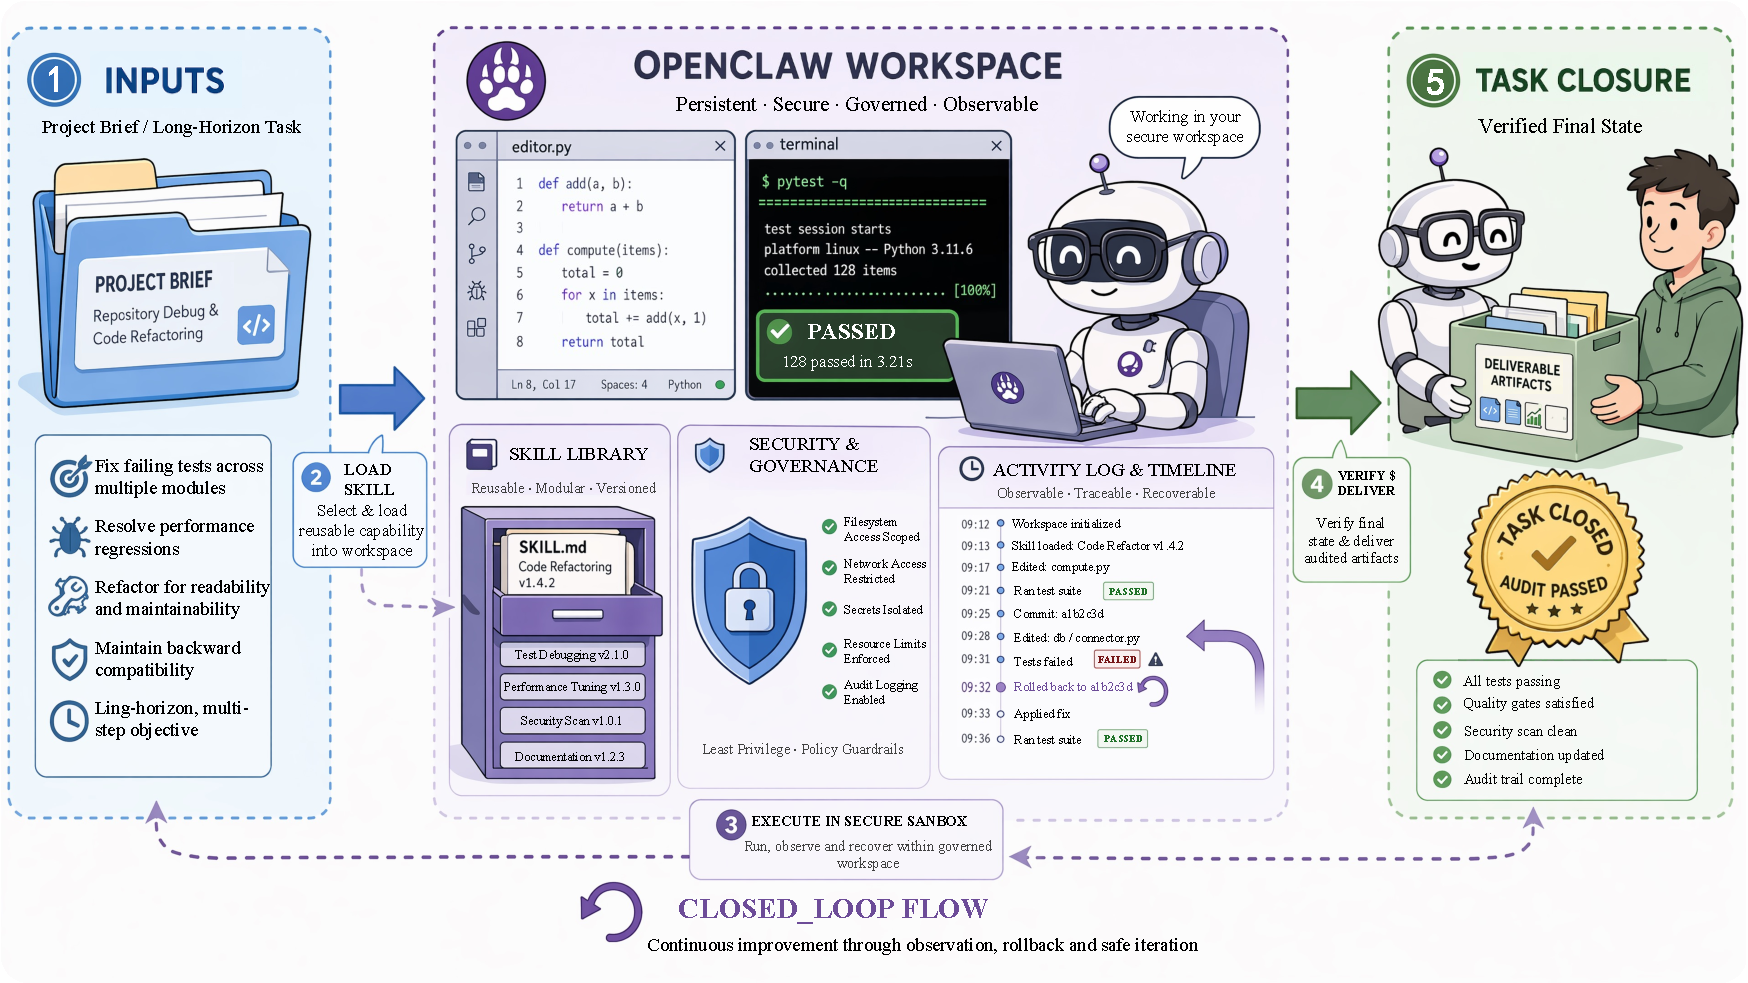
\includegraphics[width=\textwidth]{figure/openclaw.pdf}
    \caption{The OpenClaw Era: the agent works inside a persistent workspace with files, terminals, browsers, logs, permissions, reusable skills, and verification loops. The figure illustrates how workspace state and skill-based execution turn fragmented tool use into inspectable, recoverable, and deliverable task closure.}
    \label{fig:openclaw}
\end{figure}


\paragraph{Boundary from the Agent Era to the OpenClaw Era.}
As shown in Figure~\ref{fig:openclaw}, the boundary between the Agent era and the OpenClaw era is not simply whether a model can call tools.
A system belongs to the Agent era when its minimal architecture is an environment--action--feedback loop: it observes a state, reasons about the next move, invokes an external tool or action, and incorporates the returned observation into the next step.
This definition captures the first break from chatbot-style response generation, but it does not guarantee durable state, reusable procedures, recoverable execution, or final-state verification.
The environment remains something the agent queries from the outside.

By contrast, the OpenClaw era begins when the environment becomes a persistent host.
The defining condition is that agents work inside a managed workspace where files, sessions, logs, tools, project instructions, permissions, and reusable skills persist across the trajectory.
In this setting, actions are not merely tool calls; they are workspace operations whose effects can be inspected, validated, rolled back, and governed.
The conceptual unit therefore shifts from an agent that attempts a sequence of actions to a workstation system delivering a correct, auditable final state.
Table~\ref{tab:agent_openclaw_boundary} summarizes this.

\begin{table}[t]
\centering
\caption{Boundary between the Agent Era and the OpenClaw Era.}
\label{tab:agent_openclaw_boundary}
\begingroup
\footnotesize
\renewcommand{\arraystretch}{1}
\resizebox{\columnwidth}{!}{
\begin{tabular}{@{} p{0.18\columnwidth} p{0.3\columnwidth} p{0.4\columnwidth} @{}}
\toprule
\textbf{Dimension} & \textbf{Agent Era} & \textbf{OpenClaw Era} \\
\midrule
Organizing abstraction & Environment--action--feedback loop & Persistent workspace for task hosting \\
Unit of action & Tool call or external API invocation & Workspace operation over files, terminals, browsers, services, and skills \\
State model & Episodic observations and short-horizon memory & Durable files, sessions, logs, repositories, local memory, and snapshots \\
Knowledge reuse & Prompt patterns, retrieved memory, or ad-hoc demonstrations & Reusable skill packages with instructions, scripts, dependencies, examples, and checks \\
Task objective & Produce useful intermediate actions or responses & Deliver a correct, inspectable, and recoverable final workspace state \\
Evaluation focus & Action correctness and trajectory success rate & Task closure, final-state verification, repeatability, and auditability \\
Failure recovery & Best-effort retry or prompt-level reflection & Structured verification, rollback, rerun, sandboxing, and state repair \\
Safety boundary & Prompt-level guardrails and tool-use policies & Runtime permissions, provenance tracking, audit logs, and governance over workspace changes \\
\bottomrule
\end{tabular}
}
\endgroup
\end{table}

The OpenClaw era denotes the point at which agent research becomes inseparable from the workstation in which the agent is deployed.
Earlier agents mainly demonstrated that LLMs could reason, choose tools, and react to observations.
OpenClaw-style systems instead make the workspace itself the organizing abstraction: the agent is connected to persistent files, terminals, browsers, messaging channels, credentials, project instructions, local memory, and reusable skills \cite{openclaw2026repo}.
The result is a shift from \emph{tool use} to \emph{task hosting}.
An agent is no longer evaluated only by whether it emits a plausible next action, but by whether it can leave a durable, inspectable, and safe final state in a real software environment.
We therefore summarize this era along two axes: the emergence of workspace intelligence and skill-based task closure, and the new reliability, verification, and governance problems created by persistent computer use.
Table~\ref{tab:openclaw_era} summarizes representative works that define these workspace, skill, task-closure, evaluation, reliability, and governance dimensions.

\subsubsection{Workspace Intelligence and Skill-Based Task Closure}



The central architectural change is the move from isolated tool invocation to situated work inside a persistent workstation.
OpenClaw is best read as a representative engineering manifestation of this transition rather than as its sole conceptual origin: it packages a local personal assistant around a gateway, workspace, communication channels, prompt files, skills, and tool integrations \cite{openclaw2026repo}.
Related software-engineering agents show why this matters.
OpenHands provides an open platform in which agents edit code, run shell commands, browse, and execute programs inside controlled development environments \cite{wang2024openhands}.
SWE-agent further argues that the agent-computer interface is itself a decisive design object: repository navigation, file editing, command execution, and test feedback must be shaped for language-model agents rather than inherited unchanged from human-facing tools \cite{yang2024sweagent}.
Together, these systems make clear that the next step after API calling is not merely adding more tools, but constructing a stable workbench in which intermediate artifacts, environmental state, and verification signals can persist across the trajectory.

\begin{table}[t]
\centering
\scriptsize
\setlength{\tabcolsep}{1pt}
\renewcommand{\arraystretch}{1.3}
\caption{Representative works related to the OpenClaw era and workspace-level task execution.}
\label{tab:openclaw_era}
\resizebox{\columnwidth}{!}{
\begin{tabular}{@{} l l l l l @{}}
\toprule
\textbf{Work} & \textbf{Year} & \textbf{Category} & \textbf{Role} & \textbf{Key Contribution} \\
\midrule

OpenClaw~\cite{openclaw2026repo} & 2026 & Workspace & Agent Framework & Persistent workspace with tools, channels, and skills \\
OpenHands~\cite{wang2024openhands} & 2024 & Workspace & Agent Platform & Code editing, shell execution, browsing in controlled environments \\
SWE-agent~\cite{yang2024sweagent} & 2024 & Workspace & Agent-Computer Interface & Repository navigation and test-feedback interface for agents \\
SemaClaw~\cite{zhu2026semaclaw} & 2026 & Workspace & Harness Architecture & Auditable execution substrate decoupled from UI surfaces \\
Sema Code~\cite{wang2026semacode} & 2026 & Workspace & Coding Harness & Controllable workspace harness for software agents \\
Voyager~\cite{wang2023voyager} & 2023 & Skill & Agent System & Executable skill library learned from environment feedback \\
Anthropic Agent Skills~\cite{anthropic2026skillsdocs,anthropic2026skillsrepo} & 2026 & Skill & Skill Infrastructure & Folder-based skills with instructions, scripts, and resources \\
OpenClaw Skills~\cite{openclaw2026skillsdocs,openclaw2026skillsrepo} & 2026 & Skill & Skill Infrastructure & Workspace-local \texttt{SKILL.md} packages for reusable procedures \\
Awesome OpenClaw Skills~\cite{voltagent2026awesomeopenclawskills} & 2026 & Skill & Skill Repository & Public registry of reusable OpenClaw skill packages \\
Agent Skills Analysis~\cite{ling2026agentskills} & 2026 & Skill & Conceptual Analysis & Composable capability packages for data-driven agents \\
SkillFortify~\cite{bhardwaj2026skillfortify} & 2026 & Skill & Security Analysis & Metadata, dependency, provenance, and sandboxing requirements \\
SWE-bench~\cite{jimenez2023swebench} & 2024 & Task Closure & Benchmark & Real GitHub issue resolution verified by tests \\
Terminal-Bench~\cite{merrill2026terminalbench} & 2026 & Task Closure & Benchmark & Long-horizon command-line task execution \\
OSWorld~\cite{xie2024osworld} & 2024 & Evaluation & Benchmark & Real OS tasks with execution-based checking scripts \\
WebArena~\cite{zhou2023webarena} & 2023 & Evaluation & Benchmark & Realistic web environments with stateful task success \\
WorkArena~\cite{drouin2024workarena} & 2024 & Evaluation & Benchmark & Enterprise-software workflow evaluation \\
TheAgentCompany~\cite{theagentcompany2024} & 2024 & Evaluation & Benchmark & Simulated software-company work tasks \\
Reliability of Computer-Use Agents~\cite{reliability2026computeruse} & 2026 & Reliability & Reliability Study & Repeated-run instability in computer-use agents \\
Science of Agent Reliability~\cite{rabanser2026sciencereliability} & 2026 & Reliability & Reliability Agenda & Consistency, robustness, recoverability, and error severity \\
Verifiers for Computer-Use Agents~\cite{rosset2026verifiers} & 2026 & Reliability & Verification Framework & Trajectory-wide process and outcome verification \\
Your Agent Can Hurt You~\cite{wang2026youragent} & 2026 & Security & Threat Analysis & Capability, identity, and knowledge poisoning risks \\
Systematic OpenClaw Security~\cite{wang2026openclawsec} & 2026 & Security & Security Evaluation & Runtime risks beyond isolated model behavior \\
Taming OpenClaw~\cite{deng2026tamingopenclaw} & 2026 & Governance & Lifecycle Analysis & Security risks across initialization, reasoning, and execution \\
Don't Let the Claw Grip Your Hand~\cite{shan2026dontlettheclaw} & 2026 & Governance & Defense Framework & OpenClaw-specific threat modeling and defense \\
OS-Harm~\cite{kuntz2026osharm} & 2026 & Security & Safety Benchmark & Misuse, prompt injection, exfiltration, and system harm \\
OpenClaw PRISM~\cite{li2026prism} & 2026 & Governance & Defense Layer & Defense-in-depth over the OpenClaw lifecycle \\
ClawGuard~\cite{zhao2026clawguard} & 2026 & Governance & Runtime Guardrail & File, command, network, and skill boundary enforcement \\
Agentic Forensics~\cite{gruber2026agenticforensics} & 2026 & Governance & Forensics Framework & Trace reconstruction across nondeterministic agent loops \\

\bottomrule
\end{tabular}
}
\end{table}

A second defining feature is the rise of skills as modular, reusable units of agent capability.
The underlying idea predates OpenClaw: Voyager demonstrated that agents can build and reuse an executable skill library from environmental feedback \cite{wang2023voyager}.
What changes in contemporary workstation agents is that skills become file-system-level packages rather than only memories or prompt snippets.
Anthropic's Agent Skills formalize this pattern as folders containing a \texttt{SKILL.md} file, instructions, scripts, and resources that can be dynamically loaded only when relevant \cite{anthropic2026skillsdocs,anthropic2026skillsrepo}.
OpenClaw adopts a similar operational pattern through workspace-local skills organized around \texttt{SKILL.md} files and shared public skill repositories \cite{openclaw2026skillsdocs,openclaw2026skillsrepo,voltagent2026awesomeopenclawskills}.
Recent empirical analysis of Claude skills frames this development as a data-driven shift from monolithic agents toward composable capability packages \cite{ling2026agentskills}.
However, skill modularity also changes the trust model: reusable skills can encode domain expertise, but they can also become stale, over-specific, incompatible, or malicious.
Formal and supply-chain analyses of agentic skills therefore treat metadata, dependencies, versioning, provenance, and sandboxing as first-class requirements rather than engineering details \cite{bhardwaj2026skillfortify}.


The third feature is closed-loop task closure.
A workstation agent must not only plan a trajectory but also inspect the environment after each action, repair failures, rerun commands, validate outputs, and produce deliverable artifacts.
This makes reliability an emergent property of the whole harness: model, workspace, tools, skills, permission boundaries, verification scripts, and recovery policies.
Coding and terminal benchmarks make this requirement concrete.
SWE-bench evaluates whether agents can modify real repositories and pass tests for GitHub issues \cite{jimenez2023swebench}, while Terminal-Bench targets hard, realistic command-line tasks where success depends on sustained shell interaction and environment management \cite{merrill2026terminalbench}.
SemaClaw and Sema Code explicitly formulate this trend as harness engineering: the agent should be decoupled from any single user interface and embedded into a controllable, auditable execution substrate that can power IDEs, CLIs, and multi-channel personal assistants \cite{zhu2026semaclaw,wang2026semacode}.
In this sense, OpenClaw's significance lies less in a new reasoning algorithm than in productizing a complete workstation stack around the model.

\subsubsection{Evaluation, Reliability, and Governance Challenges}

Workspace intelligence also fundamentally changes what counts as evaluation. A useful workstation agent must leave the target environment in a correct, verifiable final state, not merely generate plausible reasoning. OSWorld evaluates multimodal autonomous agents in real operating-system environments with desktop applications, file operations, browsers, and execution-based checking scripts \cite{xie2024osworld}. WebArena and WorkArena extend this state-based evaluation perspective to realistic websites and complex enterprise software workflows \cite{zhou2023webarena,drouin2024workarena}. TheAgentCompany pushes the same idea toward a simulated software company environment, where agents must browse the web, write code, run programs, and communicate with coworkers to complete consequential professional work tasks \cite{theagentcompany2024}. These benchmarks show that the frontier research problem is no longer simply language understanding or isolated, single-step tool selection; it is robust long-horizon task execution in environments that are asynchronous, stateful, and only partially observable.


Recent reliability work sharpens this point.
Computer-use agents may succeed once and fail on a repeated run because execution is stochastic, task specifications are underspecified, and small environmental changes compound over long trajectories \cite{reliability2026computeruse}.
A broader reliability agenda therefore argues that single success rates should be decomposed into consistency, robustness, predictability, recoverability, and bounded error severity \cite{rabanser2026sciencereliability}.
Verification becomes a bottleneck of its own: the system must decide whether the final state actually satisfies the user intent, whether the process was safe, and whether success occurred for the right reason.
Verifier design for computer-use agents consequently emphasizes trajectory-wide evidence, the separation of process and outcome signals, and the distinction between controllable and uncontrollable failures \cite{rosset2026verifiers}.
For OpenClaw-style assistants, these findings imply that evaluation should include repeated execution, perturbation tests, state inspection, and post-hoc auditability, not only one-off demonstrations.

The same persistent workspace that enables task closure also expands the attack surface.
OpenClaw-style agents may hold credentials, local files, identity tokens, tool permissions, communication channels, and long-term memory.
Recent safety analyses show that poisoning an agent's capabilities, identity, or knowledge can turn useful autonomy into attacker-controlled authority \cite{wang2026youragent}.
Systematic security evaluations of OpenClaw and its variants further report that agentized runtimes can be riskier than the underlying models in isolation, because persistent context, orchestration, and multi-step execution amplify model weaknesses into concrete system-level failures \cite{wang2026openclawsec}.
Taming OpenClaw analyzes these risks through the lifecycle of autonomous agents, including initialization, input handling, reasoning, decision making, and execution \cite{deng2026tamingopenclaw}; Don't Let the Claw Grip Your Hand similarly proposes a defense framework for OpenClaw-specific threats \cite{shan2026dontlettheclaw}.
Beyond OpenClaw, OS-Harm shows that computer-use agents must be evaluated for misuse, indirect prompt injection, data exfiltration, and system-level harm rather than only helpfulness \cite{kuntz2026osharm}.

The security response is therefore moving from prompt-level safety toward runtime governance.
OpenClaw PRISM proposes a defense-in-depth layer over the agent lifecycle, including message ingress, prompt construction, tool execution, tool-result persistence, outbound messaging, sub-agent spawning, and gateway startup \cite{li2026prism}.
ClawGuard takes a tool-boundary view, checking file, command, network, and skill operations against user-confirmed constraints and audit policies before execution \cite{zhao2026clawguard}.
These defenses reflect a broader lesson: once an agent can act through a workstation, policy must be enforced where actions become real, not merely expressed as natural-language instructions.
Forensics becomes part of the same agenda.
Because a personal agent can modify files, invoke services, update memory, and choose tools nondeterministically over time, investigations must reconstruct traces across the entire agent loop rather than inspect a single prompt-response pair \cite{gruber2026agenticforensics}.

In summary, the OpenClaw era fundamentally reframes agentic AI as situated task execution.
Its core technological contribution is not simply broader tool access, but the integration of persistent workspaces, modular skills, closed-loop execution, verification, and runtime governance into a single harness.
The next generation of autonomous agents will therefore be differentiated not only by model scale but by the maturity of their underlying workspace stack: state management, skill provenance, permission control, repeated-execution reliability, audit trails, and safety enforcement.

\begin{AIbox}{Key Difference: From Tool Use to Task Hosting}
    \begin{itemize}[left=2pt,topsep=1pt,itemsep=2pt, parsep=1pt]
        \item OpenClaw-style systems shift the organizing abstraction from isolated API calls to persistent workspaces containing files, terminals, browsers, credentials, memory, and reusable skills.

        \item This transition makes task closure, verification, skill provenance, permission control, and runtime governance central requirements for building reliable workstation agents.
    \end{itemize}
\end{AIbox}
